\documentclass[letterpaper]{article}
%\documentclass[a5paper]{article}

%% Language and font encodings
\usepackage[english]{babel}
\usepackage[utf8x]{inputenc}
\usepackage[T1]{fontenc}

%% Sets page size and margins
\usepackage[letterpaper,top=1in,bottom=1in,left=1in,right=1in,marginparwidth=1.75cm]{geometry}
%\usepackage[a5paper,top=1cm,bottom=1cm,left=1cm,right=1.5cm,marginparwidth=1.75cm]{geometry}

%% Useful packages
\usepackage{amssymb, amsmath, amsthm} 
%\usepackage{graphicx}  %%this is currently enabled in the default document, so it is commented out here. 
\usepackage{calrsfs}
\usepackage{braket}
\usepackage{mathtools}
\usepackage{lipsum}
\usepackage{tikz}
\usetikzlibrary{cd}
\usepackage{verbatim}
%\usepackage{ntheorem}% for theorem-like environments
\usepackage{mdframed}%can make highlighted boxes of text
%Use case: https://tex.stackexchange.com/questions/46828/how-to-highlight-important-parts-with-a-gray-background
\usepackage{wrapfig}
\usepackage{centernot}
\usepackage{subcaption}%\begin{subfigure}{0.5\textwidth}
\usepackage{pgfplots}
\pgfplotsset{compat=1.13}
\usepackage[colorinlistoftodos]{todonotes}
\usepackage[colorlinks=true, allcolors=blue]{hyperref}
\usepackage{xfrac}					%to make slanted fractions \sfrac{numerator}{denominator}
\usepackage{enumitem}            
    %syntax: \begin{enumerate}[label=(\alph*)]
    %possible arguments: f \alph*, \Alph*, \arabic*, \roman* and \Roman*
\usetikzlibrary{arrows,shapes.geometric,fit}

\DeclareMathAlphabet{\pazocal}{OMS}{zplm}{m}{n}
%% Use \pazocal{letter} to typeset a letter in the other kind 
%%  of math calligraphic font. 

%% This puts the QED block at the end of each proof, the way I like it. 
\renewenvironment{proof}{{\bfseries Proof}}{\qed}
\makeatletter
\renewenvironment{proof}[1][\bfseries \proofname]{\par
  \pushQED{\qed}%
  \normalfont \topsep6\p@\@plus6\p@\relax
  \trivlist
  %\itemindent\normalparindent
  \item[\hskip\labelsep
        \scshape
    #1\@addpunct{}]\ignorespaces
}{%
  \popQED\endtrivlist\@endpefalse
}
\makeatother

%% This adds a \rewnewtheorem command, which enables me to override the settings for theorems contained in this document.
\makeatletter
\def\renewtheorem#1{%
  \expandafter\let\csname#1\endcsname\relax
  \expandafter\let\csname c@#1\endcsname\relax
  \gdef\renewtheorem@envname{#1}
  \renewtheorem@secpar
}
\def\renewtheorem@secpar{\@ifnextchar[{\renewtheorem@numberedlike}{\renewtheorem@nonumberedlike}}
\def\renewtheorem@numberedlike[#1]#2{\newtheorem{\renewtheorem@envname}[#1]{#2}}
\def\renewtheorem@nonumberedlike#1{  
\def\renewtheorem@caption{#1}
\edef\renewtheorem@nowithin{\noexpand\newtheorem{\renewtheorem@envname}{\renewtheorem@caption}}
\renewtheorem@thirdpar
}
\def\renewtheorem@thirdpar{\@ifnextchar[{\renewtheorem@within}{\renewtheorem@nowithin}}
\def\renewtheorem@within[#1]{\renewtheorem@nowithin[#1]}
\makeatother

%% This makes theorems and definitions with names show up in bold, the way I like it. 
\makeatletter
\def\th@plain{%
  \thm@notefont{}% same as heading font
  \itshape % body font
}
\def\th@definition{%
  \thm@notefont{}% same as heading font
  \normalfont % body font
}
\makeatother

%===============================================
%==============Shortcut Commands================
%===============================================
\newcommand{\ds}{\displaystyle}
\newcommand{\B}{\mathcal{B}}
\newcommand{\C}{\mathbb{C}}
\newcommand{\F}{\mathbb{F}}
\newcommand{\N}{\mathbb{N}}
\newcommand{\R}{\mathbb{R}}
\newcommand{\Q}{\mathbb{Q}}
\newcommand{\T}{\mathcal{T}}
\newcommand{\Z}{\mathbb{Z}}
\renewcommand\qedsymbol{$\blacksquare$}
\newcommand{\qedwhite}{\hfill\ensuremath{\square}}
\newcommand*\conj[1]{\overline{#1}}
\newcommand*\closure[1]{\overline{#1}}
\newcommand*\mean[1]{\overline{#1}}
%\newcommand{\inner}[1]{\left< #1 \right>}
\newcommand{\inner}[2]{\left< #1, #2 \right>}
\newcommand{\powerset}[1]{\pazocal{P}(#1)}
%% Use \pazocal{letter} to typeset a letter in the other kind 
%%  of math calligraphic font. 
\newcommand{\cardinality}[1]{\left| #1 \right|}
\newcommand{\domain}[1]{\mathcal{D}(#1)}
\newcommand{\image}{\text{Im}}
\newcommand{\inv}[1]{#1^{-1}}
\newcommand{\preimage}[2]{#1^{-1}\left(#2\right)}
\newcommand{\script}[1]{\mathcal{#1}}


\newenvironment{highlight}{\begin{mdframed}[backgroundcolor=gray!20]}{\end{mdframed}}

\DeclarePairedDelimiter\ceil{\lceil}{\rceil}
\DeclarePairedDelimiter\floor{\lfloor}{\rfloor}

%===============================================
%===============My Tikz Commands================
%===============================================
\newcommand{\drawsquiggle}[1]{\draw[shift={(#1,0)}] (.005,.05) -- (-.005,.02) -- (.005,-.02) -- (-.005,-.05);}
\newcommand{\drawpoint}[2]{\draw[*-*] (#1,0.01) node[below, shift={(0,-.2)}] {#2};}
\newcommand{\drawopoint}[2]{\draw[o-o] (#1,0.01) node[below, shift={(0,-.2)}] {#2};}
\newcommand{\drawlpoint}[2]{\draw (#1,0.02) -- (#1,-0.02) node[below] {#2};}
\newcommand{\drawlbrack}[2]{\draw (#1+.01,0.02) --(#1,0.02) -- (#1,-0.02) -- (#1+.01,-0.02) node[below, shift={(-.01,0)}] {#2};}
\newcommand{\drawrbrack}[2]{\draw (#1-.01,0.02) --(#1,0.02) -- (#1,-0.02) -- (#1-.01,-0.02) node[below, shift={(+.01,0)}] {#2};}

%***********************************************
%**************Start of Document****************
%***********************************************

%===============================================
%===============Theorem Styles==================
%===============================================

%================Default Style==================
\theoremstyle{plain}% is the default. it sets the text in italic and adds extra space above and below the \newtheorems listed below it in the input. it is recommended for theorems, corollaries, lemmas, propositions, conjectures, criteria, and (possibly; depends on the subject area) algorithms.
\newtheorem{theorem}{Theorem}
\numberwithin{theorem}{section} %This sets the numbering system for theorems to number them down to the {argument} level. I have it set to number down to the {section} level right now.
\newtheorem*{theorem*}{Theorem} %Theorem with no numbering
\newtheorem{corollary}[theorem]{Corollary}
\newtheorem*{corollary*}{Corollary}
\newtheorem{conjecture}[theorem]{Conjecture}
\newtheorem{lemma}[theorem]{Lemma}
\newtheorem*{lemma*}{Lemma}
\newtheorem{proposition}[theorem]{Proposition}
\newtheorem*{proposition*}{Proposition}
\newtheorem{problemstatement}[theorem]{Problem Statement}


%==============Definition Style=================
\theoremstyle{definition}% adds extra space above and below, but sets the text in roman. it is recommended for definitions, conditions, problems, and examples; i've alse seen it used for exercises.
\newtheorem{definition}[theorem]{Definition}
\newtheorem*{definition*}{Definition}
\newtheorem{condition}[theorem]{Condition}
\newtheorem{problem}[theorem]{Problem}
\newtheorem{example}[theorem]{Example}
\newtheorem*{example*}{Example}
\newtheorem*{counterexample*}{Counterexample}
\newtheorem*{romantheorem*}{Theorem} %Theorem with no numbering
\newtheorem{exercise}{Exercise}
\numberwithin{exercise}{section}
\newtheorem{algorithm}[theorem]{Algorithm}

%================Remark Style===================
\theoremstyle{remark}% is set in roman, with no additional space above or below. it is recommended for remarks, notes, notation, claims, summaries, acknowledgments, cases, and conclusions.
\newtheorem{remark}[theorem]{Remark}
\newtheorem*{remark*}{Remark}
\newtheorem{notation}[theorem]{Notation}
\newtheorem*{notation*}{Notation}
%\newtheorem{claim}[theorem]{Claim}  %%use this if you ever want claims to be numbered
\newtheorem*{claim}{Claim}



\pgfplotsset{compat=1.13}

\title{Math 501 \linebreak
Homework 1}
\author{Trevor Klar}

\begin{document}

\maketitle

\begin{enumerate}
\item For a set $A$, let $\{0,1\}^A$ be the set of all functions from $A$ to the two point set $\{0,1\}$. Prove that $|\{0,1\}^A|=|\powerset{A}|$.
\begin{proof}
Let $\Omega: \{0,1\}^A \to \powerset{A}$ be the following mapping: $$\Omega(f) = \{x \in A : f(x) = 1\}$$ This is to say that, for any function $f:A \to \{0,1\}$, where the set $S \subset A$  is the set such that $f(S)=\{1\}$, then $\Omega(f) = S$. 

\textbf{Claim:} $\Omega$ is a bijection, so $|\{0,1\}^A|=|\powerset{A}|$.

First, we will show that $\Omega$ is 1-1. Let $f,g:A \to \{0,1\}$ be two distinct functions. Since $f \neq g$, then there exists some $x \in A$ which maps to 1 under one function, and 0 under the other. Therefore, the set $\Omega(f) \neq \Omega(g)$, since $x$ is an element of one set, and not the other. Thus, $\Omega$ is 1-1.

Now, we will show that $\Omega$ is onto. Let $S$ be an arbitrary subset of $A$. Since the domain of $\Omega$ is $\{0,1\}^A$ (which is the set of \emph{all} functions from $A$ to $\{0,1\}$), then there exists a function $f \in \domain{\Omega}$ such that $f(S)=\{1\}$, and $f(A-S)=\{0\}$. This means that $\Omega(f)=S$, and therefore, $\Omega$ is onto.
\end{proof}

\item Prove that there is no function from a set $A$ onto $\{0,1\}^A$. 
\begin{proof}
Let $\Phi$ be a function from $A$ to $\{0,1\}^A$, and let $a$ be an arbitrary element of $A$. Then, there exist functions $f_{a_0},f_{a_1} \in \{0,1\}^A$ such that 
\[
\begin{array}{cc}
{
f_{a_0}(x)=
\begin{cases}
0 & x=a\\
1 & x\neq a \\
\end{cases}
\quad

} & {

\quad
f_{a_1}(x)=
\begin{cases}
1 & x=a\\
0 & x\neq a \\
\end{cases}
}
\end{array}
\]
This means that for every $x \in A$; $\Phi(x)$ can be either $f_{x_0}$, or $f_{x_1}$, (or neither), but not both. Therefore, whenever $\Phi$ maps an element of $A$ to a function in $\{0,1\}^A$, it always leaves at least one other function behind. Thus, $\Phi$ is not onto. 
\end{proof}

\item Let $f:X \to Y$ be a function bewteen sets $X$ and $Y$. 
\begin{enumerate}[label=(\alph*)]
\item Suppose $A \subset X$. Prove that $A \subset f^{-1}(f(A))$.
\begin{proof}
Let $x$ be an arbitrary element of $A$. Since $x \in \domain{f}$, there exists some $y \in Y$ such that $f(x)=y$. Consider the preimage of $y$; $f^{-1}(\{y\})$. Since $f(x)=y$, then $x \in f^{-1}(\{y\})$, by definition. Also, since $x \in A$ and $f(x)=y$, then $\{y\} \subset f(A)$. Therefore, $x \in f^{-1}(\{y\}) \subset f^{-1}(f(A)).$
\end{proof}
\pagebreak
\item Give an example to show $f^{-1}(f(A)) \not\subset A$.
\begin{example*} Consider the following function, $f:\{1,2,3,4\} \to \{5,6,7\}$, whose definition is given by the following figure:
\begin{center}
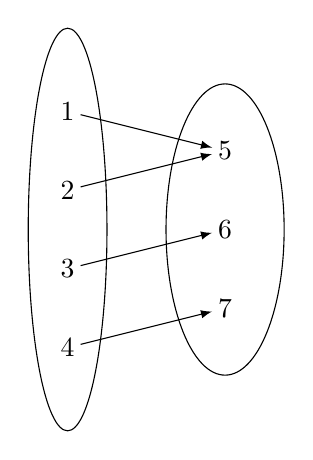
\begin{tikzpicture}
%put some nodes on the left
\foreach \x in {1,2,3,4}{
\node[inner sep=2pt] (d\x) at (0,5-\x) {\x};
}
\node[fit=(d1) (d2) (d3) (d4),ellipse,draw,minimum width=1cm] {}; 
%put some nodes on the center
\foreach \x[count=\xi] in {5,6,...,7}{
\node[inner sep=2pt] (r\xi) at (2,8.5-\x) {\x};
}
\node[fit=(r1) (r2) (r3),ellipse,draw,minimum width=1.5cm] {}; 
%put some nodes on the right
\draw[-latex] (d1) -- (r1);
\draw[-latex] (d2) -- (r1);
\draw[-latex] (d3) -- (r2);
\draw[-latex] (d4) -- (r3);
\end{tikzpicture}
\end{center}
Let $A=\{2,3,4\}$. According to the figure above, $f(A)=\{5,6,7\}$, and $f^{-1}(f(A))=\{1,2,3,4\}$. So, $f^{-1}(f(A)) \not\subset A$. \qed
\end{example*}
\item Suppose $B \subset Y$. How are the sets $B$ and $f(f^{-1}(B))$ related? Give a proof and/or example(s) to justify your answer. 

\textbf{Claim:} $f(f^{-1}(B)) \subset B$.

\begin{proof}
In the trivial case where $f^{-1}(B) = \emptyset$, $f(f^{-1}(B))$ must also be $\emptyset$, so clearly $f(f^{-1}(B)) \subset B$ and we are done. 

Now, suppose that $f^{-1}(B) \neq \emptyset$, and let $y \in f(f^{-1}(B))$. Since $y$ is in the image of $f^{-1}(B)$, there must be an $x \in f^{-1}(B)$ such that $f(x)=y$. Since $x$ is in the preimage of $B$, $f(x)$ must be in $B$. Therefore, $f(x)=y \in B$. Thus, $f(f^{-1}(B)) \subset B$.
\end{proof}

\textbf{Claim:} $B \not\subset f(f^{-1}(B))$.
\begin{example*} Consider the following function, $f:\{1,2,3\} \to \{4,5,6,7\}$, whose definition is given by the following figure:
\begin{center}
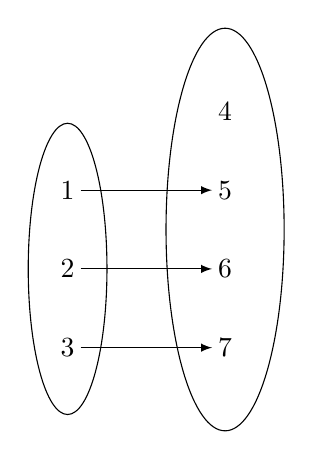
\begin{tikzpicture}
%put some nodes on the left
\foreach \x in {1,2,3}{
\node[inner sep=2pt] (d\x) at (0,4-\x) {\x};
}
\node[fit=(d1) (d2) (d3),ellipse,draw,minimum width=1cm] {}; 
%put some nodes on the center
\foreach \x[count=\xi] in {4,5,...,7}{
\node[inner sep=2pt] (r\xi) at (2,8-\x) {\x};
}
\node[fit=(r1) (r2) (r3) (r4),ellipse,draw,minimum width=1.5cm] {}; 
%put some nodes on the right
\draw[-latex] (d1) -- (r2);
\draw[-latex] (d2) -- (r3);
\draw[-latex] (d3) -- (r4);
\end{tikzpicture}
\end{center}
Let $B=\{4,5,6,7\}$. According to the figure above, $f^{-1}(B)=\{1,2,3\}$, and $f(f^{-1}(B))=\{5,6,7\}$. So, $B \not\subset f(f^{-1}(B))$.  \qed
\end{example*}
\end{enumerate}

\pagebreak
\item Give an example to show that an arbitrary (i.e. not necessarily finite) intersection of open sets in $\R^n$ need not be open. 
\begin{example*}
Consider the following set of open intervals:
$$S = \{ \left(0,\tfrac{n+1}{n}\right) : n \in \N \}.$$ 
Let $I_n$ denote the $n$th element of this set, that is, $I_n=(0,\tfrac{n+1}{n})$. Since the infimum of the set of upper bounds for these intervals is 1, 
$$\bigcap_{n=1}^{\infty}I_n=(0,1].$$
The set $(0,1]$ is not open because every open ball centered at 1 contains real numbers greater than 1, so cannot be a subset of $(0,1]$.
\qed
\end{example*}

\item Professor Doofus mistakenly writes the following on the blackboard.
\begin{romantheorem*}The following are equivalent.
\begin{enumerate}[label=(\arabic*)]
\item $f:\R^n \to \R^m$ is continuous at all $x \in \R^n$ (with the $\delta$-$\epsilon$ definition)
\item For every open set $U \subset \R^n$, the image $f(U) \subset \R^m$ is open. 
\end{enumerate}
\end{romantheorem*}
Give an example which shows why Doofus is wrong. 
\begin{example*}
Let $y \in \R^m$. Consider a constant function, $$f(x)=y, \quad \forall x \in \R^n.$$ 
The function $f$ is continuous because given any $\epsilon > 0$, we can let $\delta=1$, and if $x \in B(x_0, \delta)$, then $f(x) \in B(f(x_0), \epsilon)$ because $f(x)=f(x_0)=y$. So, (1) is true in this case. 

However, for any set $A \subset \R^n$, the image $f(A)=\{y\}$ is \emph{not} open. This is because for every $r>0$, the ball $B(y,r)$ contains points distinct from $y$, so it cannot be a subset of $\{y\}$. Therefore, (2) is false, so (1) and (2) are not equivalent statements. \qed
\end{example*}
\end{enumerate}

\end{document}